\documentclass{article}
\usepackage{amsmath}
\usepackage{mathtools}
\usepackage{gensymb}
\usepackage[a4paper,inner=1.5cm,outer=1.5cm,top=2cm,bottom=0.5cm]{geometry} 
\usepackage{xcolor}                    
\usepackage{tikz}                           
\usepackage{multicol}
\usepackage{pgfplots}
\usetikzlibrary{calc}
\usetikzlibrary{intersections}
\usetikzlibrary{intersections,calc,angles,quotes}
\usetikzlibrary{shapes,arrows,positioning,decorations.pathreplacing,calc}
\usetikzlibrary{calc,angles,positioning,intersections,quotes,decorations.markings}
\usepackage{tkz-euclide}
\usetikzlibrary{backgrounds}
\usetikzlibrary{calc,through}
\usetikzlibrary{angles}
\usetikzlibrary{fadings}
\usetikzlibrary{shapes.geometric}
\usetikzlibrary{shapes.symbols}
\usepackage{draftwatermark}
\usepackage{mathptmx}

\SetWatermarkText{\textcolor{black!10}{Mathema Shukur}}
\SetWatermarkFontSize{2 cm}
\usepackage[utf8]{inputenc}
\usepackage{fontspec}

\setmainfont{[Kalpurush.ttf]}
\newfontface{\en}{[Arial.ttf]} %%this is optional, if you want to use a secondary font. Any english font is supported
\newlength\Radius
\setlength\Radius{4cm}
\begin{document} 
	\Large
	\textcolor{red}{Welcome To} 
	\\
	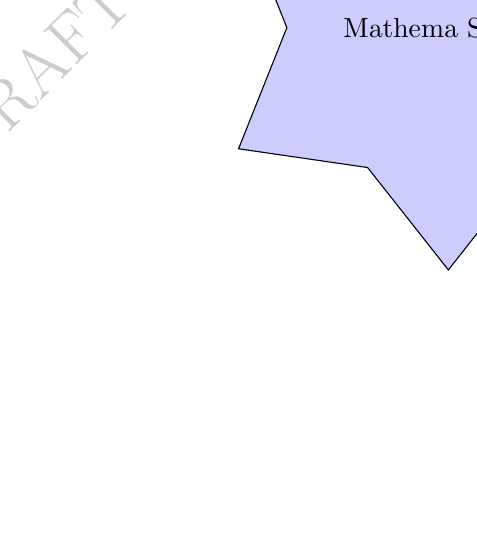
\begin{tikzpicture}
		\tikz \node [fill=blue!20,star,star points=6,draw] {Mathema Shukur };
	\end{tikzpicture}
	\\
	যাদের জন্যে প্রযোজ্যঃ  	\textcolor{magenta}{একাদশ ও দ্বাদশ শ্রেণীর শিক্ষার্থী} \\
	বিষয়ঃ \textcolor{magenta}{উচ্চতর গণিত ১ম পত্র} \\
	অধ্যায়ঃ \textcolor{magenta}{৪-বৃত্ত}\\ 
	\\
	\\
	শিখন ফলঃ\\
	(১) কেন্দ্র মূল বিন্দু বিশিষ্ট বৃত্তের সমীকরণ শনাক্ত করতে পারবে। \\
	\\
	(২)  কেন্দ্র মূল বিন্দু বিশিষ্ট বৃত্তের সমীকরণ অংকন ও অক্ষদ্বয়ের সাথে ছেদ বিন্দু নির্ধারণ করতে পারবে। \\
	\\
	(৩) নির্দিষ্ট কেন্দ্র ও ব্যাসার্ধ বিশিষ্ট বৃত্তের  সমীকরণ নির্ণয় করতে পারবে। \\
	\\
	(৪) পোলার স্থানাঙ্কে বৃত্তের  সমীকরণ নির্ণয় করতে পারবে। \\
	\\
	(৫) বৃত্তস্থ কোনো বিন্দুতে স্পর্শক ও অভিলম্বের সমীকরণ নির্ণয় করতে পারবে\\ 
	\\
	(৬) বৃত্তের বহিঃস্থ কোনো বিন্দু থেকে অঙ্কিত স্পর্শকের সমীকরণ নির্ণয় করতে পারবে\\
	\\
	(৭) বৃত্তের বহিঃস্থ কোনো বিন্দু থেকে অঙ্কিত স্পর্শকের দৈর্ঘ্য নির্ণয় করতে পারবে\\
	\\
	(৮) দুইটি বৃত্তের সাধারণ জ্যা এর সমীকরণ নির্ণয় করতে পারবে\\ 
	\\ 
	\vspace{4cm}
	\\ 
	কেন্দ্র $(h,k)$  ও ব্যাসার্ধ $r$ বিশিষ্ট বৃত্তের সমীকরণ \\ 
	\begin{align*}
		(x-h)^2+(y-k)^2&=r^2\\
		\\
		x^2-2hx+h^2+y^2-2ky+k^2&=r^2\\
		\\
		x^2+y^2-2hx-2ky+(h^2+k^2-r^2)&=0\\
		\\
		x^2+y^2+2(-h)x+2(-k)y+(h^2+k^2-r^2)&=0\\
		\\
		x^2+y^2+2gx+2fy+c&=0
	\end{align*}
\\
ধরি,\\ 
$-h=g,\,\,\Rightarrow h=-g$\\
\\
$-k=f,\,\,\Rightarrow k=-f$\\
\\
কেন্দ্র $(h,k)=(-g,-f)$\\
\\ 
ধরি,\\
$c=h^2+k^2-r^2$\\
\\
$c=g^2+f^2-r^2$\\
\\ 
$r^2=g^2+f^2-c$\\
\\ 
ব্যাসার্ধ $r=\sqrt{g^2+f^2-c}$\\
\\ 
	বৃত্তের সাধারণ সমীকরণ \\
	$\textcolor{blue}{x^2+y^2+2gx+2fy+c=0}$\\
	\\ 
	(i) এটি $x$, $y$ যুক্ত একটি দ্বিঘাত বহুপদী সমীকরণ \\
	(ii) $x^2$ এবং $y^2$ এর সহগ সমান\\
	(iii) $xy$ যুক্ত পদটি অনুপস্থিত। \\
	\\
	$c=0$ হলে বৃত্তটি মূলবিন্দু দিয়ে যাবে।\\
	\\ 
\textcolor{blue}{কেন্দ্রের স্থানাঙ্ক	$(-g,-f)$}\\
\\
$g=0$ হলে কেন্দ্র $y-$অক্ষের উপর অবস্থিত\\
\\
$f=0$ হলে কেন্দ্র $x-$  অক্ষের উপর অবস্থিত\\ 
\\ 
\textcolor{blue}{ব্যাসার্ধ	$\sqrt{g^2+f^2-c}$}\\
\\
যদি $g^2+f^2-c=0$ হয়, তাহলে বৃত্তের ব্যাসার্ধ শূন্য হবে এবং এক্ষেত্রে বৃত্তটি  $(-g,-f)$ বিন্দুতে পরিনত হবে। এরুপ বৃত্তকে বিন্দু বৃত্ত বলে। \\
\\ 
\textcolor{red}{$x^2+y^2+2gx+2fy+c=0$, $(g^2>c\,\,\,f^2>c)$ বৃত্তটি দ্বারা অক্ষ দুইটি থেকে ছেদিত অংশের পরিমান নির্ণয় কর। }\\
\\
মনে করি, বৃত্তটি $x-$ অক্ষকে $(x_1,0)$ও $(x_2,0)$ বিন্দুতে ছেদ করে। \\
\\
বৃত্তের সাধারণ সমীকরণে $y=0$ বসিয়ে পাই $x^2+2gx+c=0$\\
\\
$x_1$ ও $x_2$ উপরের সমীকরণটির মূল হবে। \\
\\
মূলদ্বয়ের যোগফল $x_1+x_2=-2g$\\
\\
মূলদ্বয়ের গুনফল $x_1\,\,x_2=c$\\
\\
বৃত্তটি দ্বারা $x-$ অক্ষের ছেদিত অংশের পরিমান \\ 
\begin{align*}
&|x_1-x_2|\\
\\
&=\sqrt{(x_1-x_2)^2}\\
\\
&=\sqrt{(x_1-x_2)^2-4x_1\,x_2}\\
\\
&=\sqrt{4g^2-4c}\\
\\
&=2\sqrt{g^2-c}	
\end{align*} 
\\
বৃত্তের সাধারণ সমীকরণে $x=0$ বসিয়ে পাই $y^2+2fy+c=0$\\
\\
$y_1$ ও $y_2$ উপরের সমীকরণটির মূল হবে। \\
\\
মূলদ্বয়ের যোগফল $y_1+y_2=-2f$\\
\\
মূলদ্বয়ের গুনফল $y_1\,\,y_2=c$\\
\\
বৃত্তটি দ্বারা $y-$ অক্ষের ছেদিত অংশের পরিমান \\ 
\begin{align*}
	&|y_1-y_2|\\
	\\
	&=\sqrt{(y_1-y_2)^2}\\
	\\
	&=\sqrt{(y_1-y_2)^2-4y_1\,y_2}\\
	\\
	&=\sqrt{4f^2-4c}\\
	\\
	&=2\sqrt{f^2-c}	
\end{align*} 
বৃত্ত দ্বারা $x$ অক্ষের খন্ডিত অংশ	$2\sqrt{g^2-c}$\\
\\
বৃত্ত যদি $x-$ অক্ষকে স্পর্শ করে তবে $x-$ অক্ষের ছেদিত অংশের মান শূন্য হবে  \\
$2\sqrt{g^2-c}=0$\\
 $g^2=c$\\
\\
বৃত্তটি  $x$ অক্ষকে স্পর্শ করলে  $g^2=c$\\
\\
বৃত্ত দ্বারা $y$ অক্ষের খন্ডিত অংশ	$2\sqrt{f^2-c}$\\
 \\
 বৃত্ত যদি $y-$ অক্ষকে স্পর্শ করে তবে $y-$ অক্ষের ছেদিত অংশের মান শূন্য হবে\\
   $2\sqrt{f^2-c}=0$\\
    $f^2=c$\\
 \\ 
বৃত্তটি  $y$ অক্ষকে স্পর্শ করলে  $f^2=c$\\
\\
বৃত্তটি উভয় অক্ষকে স্পর্শ করলে 	$g^2=f^2=c$\\ 
\\
\textcolor{blue}{[ঢাকা বিশ্ববিদ্যালয় ভর্তি পরীক্ষা -২০১৪-২০১৫]}\\
$kx^2+2y^2-4x-12y+11=0$ সমীকরণটি বৃত্ত নির্দেশ করলে k এর মান কত ? \\ 
\\
\textcolor{blue}{[KUET-2011-2012]}\\
k এর কোন মানের জন্য  $(x-y+3)^2+(kx+2)(y-1)=0$ সমীকরণটি একটি বৃত্ত নির্দেশ করে। \\ 
\\ 
\textcolor{blue}{[কুমিল্লা বোর্ড-২০২২]}\\
$ax^2+by^2=c$ সমীকরণটি একটি বৃত্ত নির্দেশ করলে $a$ ও $b$ এর মধ্যে সম্পর্ক কী হবে ?  \\
\\ 
\textcolor{blue}{[কুমিল্লা বোর্ড-২০২২]}\\
$2x^2+2y^2+4x-2y+4=0$ বৃত্তের কেন্দ্র নির্ণয় কর \\ 
\\
\textcolor{blue}{[ঢাকা বিশ্ববিদ্যালয় ভর্তি পরীক্ষা -২০১৮-২০১৯]}\\
$3x^2+3y^2-5x-6y+4=0$ বৃত্তের কেন্দ্র নির্ণয় কর \\ 
\\
\textcolor{blue}{[ চট্রগ্রাম বিশ্ববিদ্যালয় ভর্তি পরীক্ষা -২০১৪-২০১৫]}\\
$x^2+y^2-24x+10y=0$ বৃত্তের ব্যাসার্ধ নির্ণয় কর \\ 
\\
\textcolor{blue}{[ নোয়াখালী বিজ্ঞান ও প্রযুক্তি বিশ্ববিদ্যালয় ভর্তি পরীক্ষা -২০১৭-২০১৮]}\\
$2x^2+2y^2-4x-12y+11=0$ বৃত্তের ব্যাসার্ধ নির্ণয় কর \\ 
\\
\textcolor{blue}{[দিনাজপুর বোর্ড-২০২২]}\\
$3x^2+3y^2-6x+4y-1=0$ বৃত্তের কেন্দ্র নির্ণয় কর \\ 
\\
\textcolor{blue}{[ঢাকা বোর্ড-২০২২]}\\
$x^2+y^2-6x+8y+9=0$ বৃত্ত দ্বারা $y-$  অক্ষের খন্ডিত অংশের পরিমান নির্ণয় কর \\ 
\\
\textcolor{blue}{[ঢাকা বোর্ড-২০২২]}\\
$3x^2+3y^2-6x-9y-3=0$ বৃত্ত দ্বারা $x-$  অক্ষের খন্ডিত অংশের পরিমান নির্ণয় কর \\ 
\\
\textcolor{blue}{[CUET-2010-2011]}\\
$k$ এর কোন মানের জন্য  $x^2+y^2+kx+2y+25=0$ বৃত্তটি $x-$ অক্ষকে স্পর্শ করে \\ 
\\ 
\textcolor{blue}{[বরিশাল বোর্ড-২০২২]}\\
 যদি $x^2+y^2-12x+8y+c=0$ বৃত্তটি $x-$ অক্ষকে স্পর্শ করে তবে  $c$ এর মান নির্ণয় কর। স্পর্শ বিন্দুর স্থানাঙ্ক নির্ণয় কর। \\
 \\ 
 \textcolor{blue}{[সিলেট বোর্ড-২০২২]}\\
 যদি $x^2+y^2-4x-6y+c=0$ বৃত্তটি $y-$ অক্ষকে স্পর্শ করে তবে  $c$ এর মান নির্ণয় কর।স্পর্শ বিন্দুর স্থানাঙ্ক নির্ণয় কর। \\
 \\ 
 \textcolor{blue}{[রাজশাহী বোর্ড-২০২২]}\\
 $x^2+y^2-4x-6y=7$ বৃত্ত দ্বারা $x-$  অক্ষের খন্ডিত অংশের পরিমান নির্ণয়  কর \\ 
 \\
 \textcolor{blue}{[যশোর বোর্ড-২০২২]}\\
 $x^2+y^2-2x+6y-6=0$ বৃত্ত দ্বারা $x-$  অক্ষের খন্ডিত অংশের দৈর্ঘ্য নির্ণয়  কর \\ 
 \\
 \textcolor{blue}{[দিনাজপুর বোর্ড-২০২২]}\\
 $x^2+y^2+4x-6y-1=0$ বৃত্ত দ্বারা $y-$  অক্ষের খন্ডিত অংশের পরিমান  কর \\ 
 \\
  \textcolor{blue}{[কুমিল্লা বোর্ড-২০২২]}\\
 $x^2+y^2-4x+8y=0$ বৃত্ত দ্বারা $y-$  অক্ষের খন্ডিত অংশের দৈর্ঘ্য নির্ণয়  কর \\ 
 \\
	কেন্দ্র  $C(h,k)$ বিন্দুতে এবং ব্যাসার্ধ $r$ বিশিষ্ট বৃত্ত। কেন্দ্র থেকে পরিধির উপর অবস্থিত $A(x,y)$ বিন্দুর দূরত্ব হলো ব্যাসার্ধ। \\ 
	\\ 
	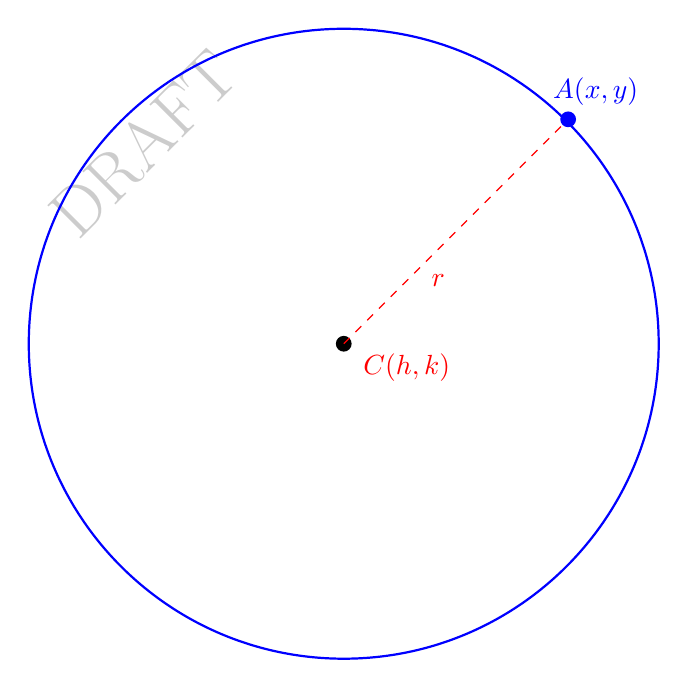
\begin{tikzpicture}[transform shape,scale=1]
		\fill[black] (0,0) circle (1 mm);
		\node at (0.8,-0.3) {$\textcolor{red}{C(h,k)}$};	
		\draw[thick,blue] (0,0) circle (4);
		\draw[dashed,red] (0,0)--(2.8,2.8);
		\node at (3.2,3.2) {$\textcolor{blue}{A(x,y)}$};	
		\fill[blue] (2.85,2.85) circle (1 mm);
		\node at (1.2,0.8) {$\textcolor{red}{r}$};		
	\end{tikzpicture}\\
	\\
	\begin{align*}
		AC&=r\\
		\\
		\sqrt{(x-h)^2+(y-k)^2}&=r\\
		\\
		(x-h)^2+(y-k)^2&=r^2
	\end{align*}
	\\
	\\
	$(h,k)$ কেন্দ্র ও $r$  ব্যাসার্ধ  বিশিষ্ট বৃত্তের সমীকরণ \\
	\\
	$\textcolor{blue}{(x-h)^2+(y-k)^2=r^2}$\\
	\\
	\vspace{7cm}
	\\
	\textcolor{red}{[দিনাজপুর বোর্ড-২০২২]}\\
	$(-2,3)$ বিন্দুতে কেন্দ্র এবং $y-$ অক্ষকে স্পর্শ করে এরুপ বৃত্তের সমীকরণ নির্ণয় কর \\
	\\
	\begin{tikzpicture}[transform shape,scale=1]
		\draw [-latex,thick,red](-6,0) -- (6,0) node[right] {$x$} coordinate(x axis);
		\draw [-latex,thick,red](0,-6) -- (0,6) node[above] {$y$} coordinate(y axis);
		\fill[black] (0,0) circle (1 mm);
		\node at (0.8,-0.3) {$\textcolor{red}{O(0,0)}$};	
		\draw[thick,blue] (-2,3) circle (2);
		\fill[blue] (-2,3) circle (1 mm);
		\node at (-2,2.5) {$\textcolor{blue}{(-2,3)}$};
	\end{tikzpicture}\\
	\\
	কেন্দ্র $(h,k)=(-2,3)$ ও ব্যাসার্ধ  $r=|-2|=2$\\
	\\
	\begin{align*}
		(x-h)^2+(y-k)^2&=r^2\\
		\\
		(x-(-2))^2+(y-3)^2&=2^2\\
		\\
		(x+2)^2+(y-3)^2&=4\\
	\end{align*}
	\\
	\vspace{5cm}
	\\
	\textcolor{red}{[দিনাজপুর বোর্ড-২০২২]}\\
	$(6,-4)$ বিন্দুতে কেন্দ্র এবং $x-$ অক্ষকে স্পর্শ করে এরুপ বৃত্তের ব্যাসের মান কত?  \\
	\\
	\begin{tikzpicture}[transform shape,scale=1]
		\draw [-latex,thick,red](-2,0) -- (10,0) node[right] {$x$} coordinate(x axis);
		\draw [-latex,thick,red](0,2) -- (0,-10) node[above] {$y$} coordinate(y axis);
		\fill[black] (0,0) circle (1 mm);
		\node at (0.8,-0.3) {$\textcolor{red}{O(0,0)}$};	
		\draw[thick,blue] (6,-4) circle (4);
		\fill[blue] (6,-4) circle (1 mm);
		\node at (6,-4.5) {$\textcolor{blue}{(6,-4)}$};
	\end{tikzpicture}\\
	\\ 
	ব্যাসার্ধ $r=|-4|=4$\\
	\\
	ব্যাস $2r=2\times 4=8$\\
	\\ 
	\vspace{10cm}
	\\
	\textcolor{red}{[যশোর বোর্ড-২০২২]}\\
	$(1,3)$ কেন্দ্র বিশিষ্ট বৃত্ত  $y-$ অক্ষকে স্পর্শ করে এরুপ বৃত্তের সমীকরণ নির্ণয় কর ?  \\
	\\
	\begin{tikzpicture}[transform shape,scale=1]
		\draw [-latex,thick,red](-6,0) -- (6,0) node[right] {$x$} coordinate(x axis);
		\draw [-latex,thick,red](0,-6) -- (0,6) node[above] {$y$} coordinate(y axis);
		\fill[black] (0,0) circle (1 mm);
		\node at (0.8,-0.3) {$\textcolor{red}{O(0,0)}$};	
		\draw[thick,blue] (1,3) circle (1);
		\fill[blue] (1,3) circle (1 mm);
		\node at (1,2.5) {$\textcolor{blue}{(1,3)}$};
	\end{tikzpicture}\\
	\\
	কেন্দ্র $(h,k)=(1,3)$ ও ব্যাসার্ধ  $r=1$\\
	\\
	\begin{align*}
		(x-h)^2+(y-k)^2&=r^2\\
		\\
		(x-1)^2+(y-3)^2&=1^2\\
		\\
		(x-1)^2+(y-3)^2&=1\\
	\end{align*}
	\\
	\vspace{5cm}
	\\
	\textcolor{red}{[বরিশাল বোর্ড-২০২২]}\\
	$(4,-5)$ কেন্দ্র বিশিষ্ট বৃত্ত  $x-$ অক্ষকে স্পর্শ করলে বৃত্তের ব্যাস নির্ণয় কর ?  \\
	\\
	\begin{tikzpicture}[transform shape,scale=1]
		\draw [-latex,thick,red](-3,0) -- (10,0) node[right] {$x$} coordinate(x axis);
		\draw [-latex,thick,red](0,1) -- (0,-10) node[above] {$y$} coordinate(y axis);
		\fill[black] (0,0) circle (1 mm);
		\node at (0.8,-0.3) {$\textcolor{red}{O(0,0)}$};	
		\draw[thick,blue] (4,-5) circle (5);
		\fill[blue] (4,-5) circle (1 mm);
		\node at (4,-5.5) {$\textcolor{blue}{(4,-5)}$};
	\end{tikzpicture}\\
	\\ 
	ব্যাসার্ধ $r=|-5|=5$\\
	\\
	ব্যাস $2r=2\times 5=10$\\
	\\
	\vspace{15cm}
	\\
	নিচের চিত্রানুযায়ী বৃত্তের সমীকরণ লিখ \\ 
	\begin{tikzpicture}[transform shape,scale=1]
		\draw [-latex,thick,red](-10,0) -- (2,0) node[right] {$x$} coordinate(x axis);
		\draw [-latex,thick,red](0,-10) -- (0,2) node[above] {$y$} coordinate(y axis);
		\fill[black] (0,0) circle (1 mm);
		\node at (0.8,-0.3) {$\textcolor{red}{O(0,0)}$};	
		\draw[thick,blue] (-4,-3) circle (4);
		\fill[blue] (-4,-3) circle (1 mm);
		\node at (-4,-3.7) {$\textcolor{blue}{(-4,-3)}$};
	\end{tikzpicture}\\
	\\
	\\
	\\
	\begin{tikzpicture}[transform shape,scale=1]
		\draw [-latex,thick,red](-10,0) -- (1,0) node[right] {$x$} coordinate(x axis);
		\draw [-latex,thick,red](0,-8) -- (0,1) node[above] {$y$} coordinate(y axis);
		\fill[black] (0,0) circle (1 mm);
		\node at (0.8,-0.3) {$\textcolor{red}{O(0,0)}$};	
		\draw[thick,blue] (-5,-2) circle (2);
		\fill[blue] (-5,-2) circle (1 mm);
		\node at (-5,-2.7) {$\textcolor{blue}{(-5,-2)}$};
	\end{tikzpicture}\\
\end{document}